\section{Introduction} \label{sec:introduction}
\label{sec:introduction}
%$$$$$$$$$$$$$$$$$$$$$$$$$$$$$$$$$$$$$$$$$$$$$$$$$$$$$$$$$$$$$$$$$$$$$$$$$$$$$$$$
%$$$$$$$$$$$$$$$$$$$$$$$$$$$$$$$$$$$$$$$$$$$$$$$$$$$$$$$$$$$$$$$$$$$$$$$$$$$$$$$$
%Background : 스파크 -> cloud가 아닌 scale-up server 에서의 scalability에 대한 연구가 필요해짐
%$$$$$$$$$$$$$$$$$$$$$$$$$$$$$$$$$$$$$$$$$$$$$$$$$$$$$$$$$$$$$$$$$$$$$$$$$$$$$$$$
%빅데이터 처리하는데 많이 사용되는 framework 중 하나는 스파크이다.
Scale-out and scale-up configurations are two different representative methods to implement 
big data analytics infrastructures. 
In scale-out server clusters(e.g, Spark~\cite{Zaharia2012RDD},
Hadoop~\cite{Shvachko2010HDF}), server upgrades are performed through adding nodes to 
the existing cluster system. 
On the other hand, in scale-up environment, server upgrades are performed 
through adding resources(e.g, CPU, memory) to the existing single node-based system.
Scale-up servers are mostly used in scientific analytics areas~\cite{Chaimov2016SSH}, 
and big data analytics frameworks are being increasingly used.
Another reason that the scale-up servers are becoming more popular is due to 
significantly increased resources even on single-node based server system~\cite{Appuswamy2013SVS}.
This naturally requires substantial research on how to improve the performance 
scalability of scale-up servers.

%$$$$$$$$$$$$$$$$$$$$$$$$$$$$$$$$$$$$$$$$$$$$$$$$$$$$$$$$$$$$$$$$$$$$$$$$$$$$$$$$
%$$$$$$$$$$$$$$$$$$$$$$$$$$$$$$$$$$$$$$$$$$$$$$$$$$$$$$$$$$$$$$$$$$$$$$$$$$$$$$$$
%Problem : scale-up server에서 시스템으로 구성된 scalability가 없음 
% 2가지 관련 연구가 있음.
% 1. 24코어 이하의 서버에서의 Scalability 분석을 하였으나 해결책을 제안하지 않았음.
% 2. HPC(100이상) 으로 분석하였으나 flie system 관점으로 분석하였음.:메인 병목지점은 파일 시스템
% 3. Scalable한 파일 시스템을 사용한 후 Scalability에 대한 분석한 결과와 해결방법은 없음.
Spark is one of widely used big data analytics framework.
However, Spark has been reported that it does
not scale on the single node scale-up server because of garbage
collection(GC)
overheads~\cite{Ahsan2016SVS}~\cite{Ousterhout2015MSP}~\cite{Maas2016THL} and
locality of memory accesses on Non-Uniform Memory Access(NUMA)
architecture~\cite{Cao2016ADS}.
In order to minimize the remote memory access costs, researchers have
attempted to create a new NUMA balancing~\cite{Dashti2013TMH}~\cite{AutoNUMA} and 
accomplished considerable level of performance improvement, but not satisfiable in 
scalability aspects. 

%$$$$$$$$$$$$$$$$$$$$$$$$$$$$$$$$$$$$$$$$$$$$$$$$$$$$$$$$$$$$$$$$$$$$$$$$$$$$$$$$
%본 연구에서 분석한 결과와 제안하는 방법으로 향상된 성능
%$$$$$$$$$$$$$$$$$$$$$$$$$$$$$$$$$$$$$$$$$$$$$$$$$$$$$$$$$$$$$$$$$$$$$$$$$$$$$$$$
%$$$$$$$$$$$$$$$$$$$$$$$$$$$$$$$$$$$$$$$$$$$$$$$$$$$$$$$$$$$$$$$$$$$$$$$$$$$$$$$$
In order to achieve the performance scalability, we need to devise a framework to avoid 
the major drawbacks of the Apache Spark regarding GC and remote memory access overheads.
Our proposed architecture is based on the reasoning that logically partitioning the original 
servers into small servers could hide the Spark's performance scalability problems. 
Therefore, we propose a Docker container-based logical partitioning method for Spark-based
scale-up servers. 
In this paper, we implemented a proof-of-concept architecture using Docker container-based
scale-up server while leaving concrete and detailed complete design and implementation of 
necessary server components to future work.

%Our goals is to reduce the GC and the remote memory access overheads that
%have been major problems of Spark scalability.
%To achieve our goal, this paper evaluate Docker container-based partitioning
%that eliminates the GC and remote access overheads, and present a towards
%framework to mitigate the scale-up server scalability problems.
To evaluate our approach, we manually applied our partitioning method to a 120
core scale-up server.
While smaller sized partitioning may further reduce GC overhead and remote memory access,
this may cause straggler tasks
problem~\cite{Ousterhout2015MSP}~\cite{Ren2015HDS}.
Thus, this paper additionally addresses the trade-off relationship between 
the achieved performance scalability and partitioning sizes.
Performance evaluation of the proposed best-fit partitioning on a 120 core system
 reveals that the execution times could be improved by 1.6x, 1.7x, 1.5x and 1.1x
 for Word Count, Naive Basian, Grep and K-means, respectively.

%Our basic key idea is that a shared-memory system is dealt with as a 
%distributed system using the partitioning approach in order to eliminate GC and
%memory access overheads.
%We use Docker containers since the overheads of Docker container are much smaller
%than a traditional virtual
%machine~\cite{Merkel2014DLL} and the container-based approach can easily combine
%the existing container management solutions such as Google Borg~\cite{Borg} and
%Kubernets~\cite{Kubernetes}.



%$$$$$$$$$$$$$$$$$$$$$$$$$$$$$$$$$$$$$$$$$$$$$$$$$$$$$$$$$$$$$$$$$$$$$$$$$$$$$$$$
%본 연구에서 기여한 것 : 
% 1. 100코어 이상의 scale-up 서버에서의 scalability 측정 및 분석
% 2. 도커 파티션 기법을 활용한 scalability 향상 방법 제안
%$$$$$$$$$$$$$$$$$$$$$$$$$$$$$$$$$$$$$$$$$$$$$$$$$$$$$$$$$$$$$$$$$$$$$$$$$$$$$$$$

\textbf{Contributions.} Our research provides the following contributions:
\begin{itemize}
\item 
We measured Apache Spark performance scalability on a 120 core scale-up server.
The results show that parallel GC only scales well up to 60 core systems while
does not show performance improvement on the systems with more than 60 cores.
\item 
We evaluated proposed partitioning approach on a large scale-up server
using 
BigDataBench~\cite{wang2014bigdatabench} and
the results revealed that the proposed framework significantly mitigate the 
performance scalability problems of Apache Spark.
\item 
We present a proof-of-concept architecture for Apache Spark-based scale-up servers
based on Docker-based logical partitioning.
\end{itemize}


\begin{figure*}[tb]
    \centering
    \begin{subfigure}[b]{0.25\textwidth}
        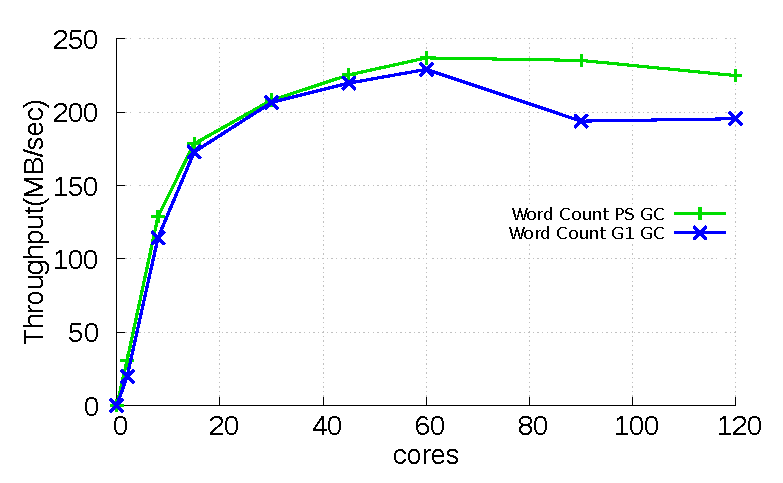
\includegraphics[width=1.8in]{graph/wc.eps}
        \caption{Word Count}
    \end{subfigure}%
    \begin{subfigure}[b]{0.25\textwidth}
        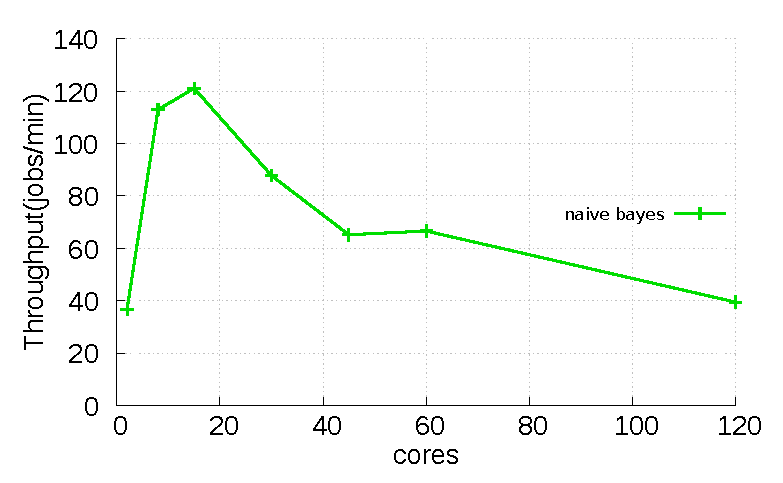
\includegraphics[width=1.8in]{graph/nb.eps}
        \caption{Naive Basian}
    \end{subfigure}%
    \begin{subfigure}[b]{0.25\textwidth}
        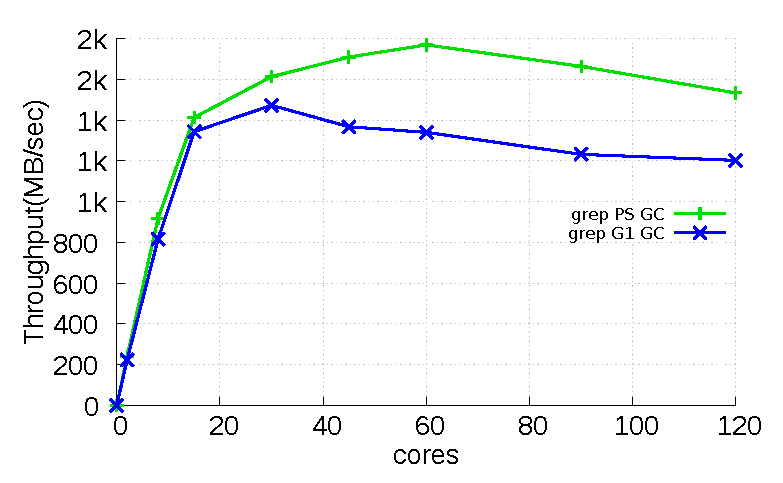
\includegraphics[width=1.8in]{graph/grep.eps}
        \caption{Grep}
    \end{subfigure}%
    \begin{subfigure}[b]{0.25\textwidth}
        \includegraphics[width=1.8in]{graph/kmeans.eps}
        \caption{K-means}
    \end{subfigure}%
    \caption{Performance scalability.}
    \label{fig:scalability}
\end{figure*}



\begin{figure*}[tb]
    \centering
    \begin{subfigure}[b]{0.25\textwidth}
        \includegraphics[width=1.8in]{graph/wc_cpuutils.eps}
        \caption{Word Count}
    \end{subfigure}%
    \begin{subfigure}[b]{0.25\textwidth}
        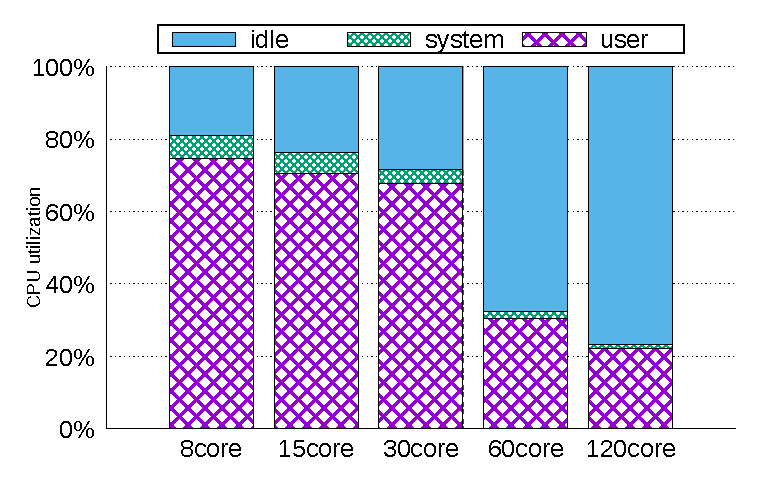
\includegraphics[width=1.8in]{graph/nb_cpuutils.eps}
        \caption{Naive Basian}
    \end{subfigure}%
    \begin{subfigure}[b]{0.25\textwidth}
        \includegraphics[width=1.8in]{graph/grep_cpuutils.eps}
        \caption{Grep}
    \end{subfigure}%
    \begin{subfigure}[b]{0.25\textwidth}
        \includegraphics[width=1.8in]{graph/kmeans_cpuutils.eps}
        \caption{K-means}
    \end{subfigure}%
        \centering
    \caption{CPU utilization.}
    \label{fig:cpuutilization}
\end{figure*}

%$$$$$$$$$$$$$$$$$$$$$$$$$$$$$$$$$$$$$$$$$$$$$$$$$$$$$$$$$$$$$$$$$$$$$$$$$$$$$$$$
%$$$$$$$$$$$$$$$$$$$$$$$$$$$$$$$$$$$$$$$$$$$$$$$$$$$$$$$$$$$$$$$$$$$$$$$$$$$$$$$$
%Mapping
%$$$$$$$$$$$$$$$$$$$$$$$$$$$$$$$$$$$$$$$$$$$$$$$$$$$$$$$$$$$$$$$$$$$$$$$$$$$$$$$$
The rest of this paper is organized as follows.
Section 2 describes the test-bed, Spark scalability problem and benefits of partitioning.
Section 3 shows the our proof-of-concept architecture.
Section 4 describes related works. 
Finally, section 5 concludes the paper.

